\addtocontents{toc}{\protect\newpage}
\chapter{Юридично-документальний рівень}

\section{Вступ}

Друге видання КНИГИ ERP (англ. ERP BOOK VOL.3 Blue Book) визначає формальну
бізнес специфікацію та її імплементацію для сучасних оптимізованих підприємств.
Системи ERP на її базі також уже не один рік використовується у банківській сфері,
процесінгу транзакцій, розподілених системах повідомлень, в IoT секторі.

\section{Модулі підприємства}

ERP/1 є комплексом бібліотек (N2O.DEV) та підсистем додатків (ERP/1),
який використовує загальну шину і загальну розподілену базу даних для швидкіснх операційних вітрин.
\\
\\
\textbf{ERP} — Даний модуль обліково-реєстраційного рівня зберігає основну ієрархічну структуру
        підприємства, її схему, метаінформацію про типи даних, а також сам інформіцію:
        записи про персонал, інвентар, компанії та офіси підприємства.
\\
\\
\textbf{CRM} — Система управління зв'язками з громадськістю та органами виконавчої влади:
        являє собою базову реалізацію постанови \#55 КМУ.
\\
\\
\textbf{CART} — Система управління клієнтами: являє собою розширення більш
           абстрактного додатку CHAT.

\newpage
\section{Управління ресурсами}

Головним чином інформаційна структура нашого підприємства
складається з обчислювальних ресурсов (додатки, запущені в шині)
та накопичувальних ресурсів (дані, збережені в базі даних).
\
\\
SOA архітектура в якості моделі управління обчислювальними
ресурсами пропонує асинхронний протокол віддаленого виклику на шинах.
Разом з N2O можно використовувати MQTT та інші шини, за допомогою наступних протоколів: TCP, WebSocket.
Ці асинхронні протоколи часто називають
протоколами реального часу, оскільки в них функції відправки повідомлень завжди
миттєво повертають результат. Що ж стосується протоколів для публікації і доступу
до даних, то тут може виявитися доречним використання синхронного HTTP протоколу.

\newpage
\section{Архітектура CRM системи}

\subsection{Сторінки}

Перелік сторінок

\begin{lstlisting}
def route(<<"ldap", _::binary>>), do: LDAP.Index
def route(<<"crm",  _::binary>>), do: CRM.Index
def route(<<"rmk",  _::binary>>), do: RMK.Index
def route(<<"kvs",  _::binary>>), do: KVS.Index
def route(<<"act",  _::binary>>), do: BPE.Actor
def route(<<"help", _::binary>>), do: HELP.Index
\end{lstlisting}

\subsubsection{LDAP}

Сторінка авторизації користувачів.

\begin{figure}[!htbp]
\centerline{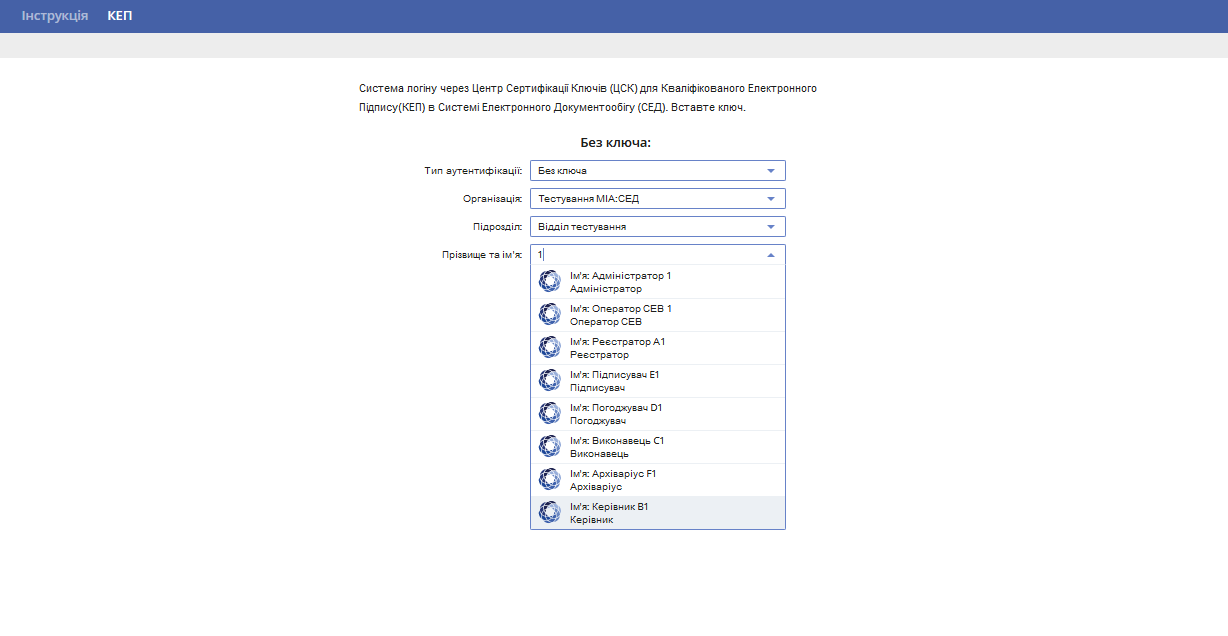
\includegraphics[scale=0.25]{LDAP.PNG}}
\caption{Сторінка авторизації}
\end{figure}

\subsection{Комболукап}

\subsection{Сервіси}

\subsection{СЕВ ОВВ}

\subsection{Шаблони}

\subsection{Дерева}

\newpage
\subsection{Процеси}

Даний модуль інкапсулює визначення Схеми, Бізнес-Процесів та Форм,
які використовуються у системі Infotech-ERP згідно методології фреймворку Захмана.

\subsubsection{Формування нормативно-довідкової інформації}

Виділяються наступні основні процеси організаційно-розпорядчих
документів: «Накази», «Протоколи», «Доручення керівництва».

\subsubsection{Обробка вхідних документів}

Вхідні документи надходять в УДСД, ВОРЗГ та ВОДПІ.
При надходженні документа уповноважена посадова особа зазначених
СП реєструє його в системі та виконується його подальша обробка.

\begin{figure}[!htbp]
\centerline{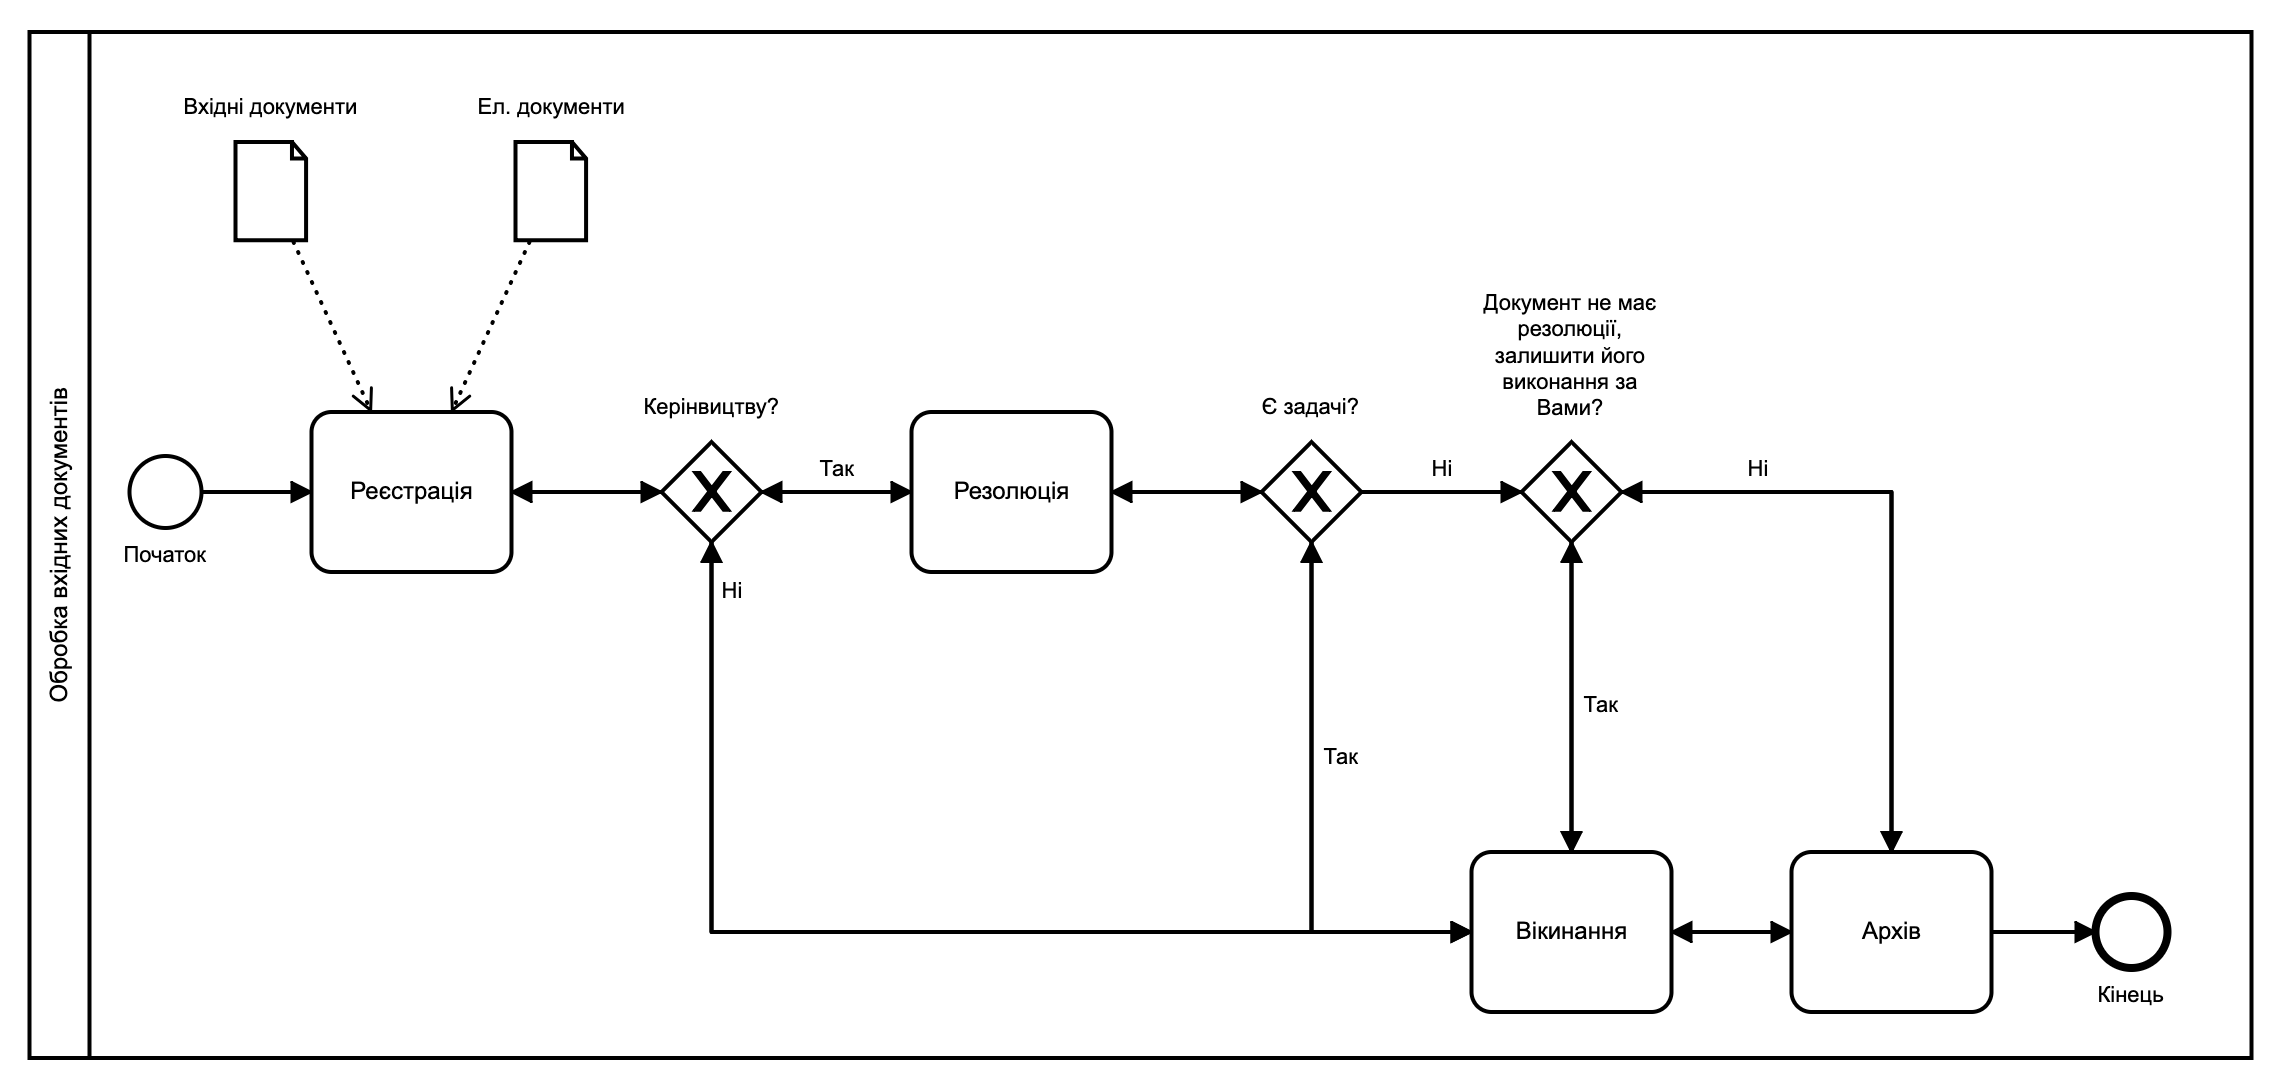
\includegraphics[scale=0.25]{handleInputDoc.png}}
\caption{Бізнес-процес обробки вхідних докумнетів}
\end{figure}

Далі вхідний документ надходить або Міністру/Заст. Міністра/Державному
секретарю для накладання резолюції, або до СП на виконання.

\subsubsection{Вхідні документи}

\begin{figure}[!htbp]
\centerline{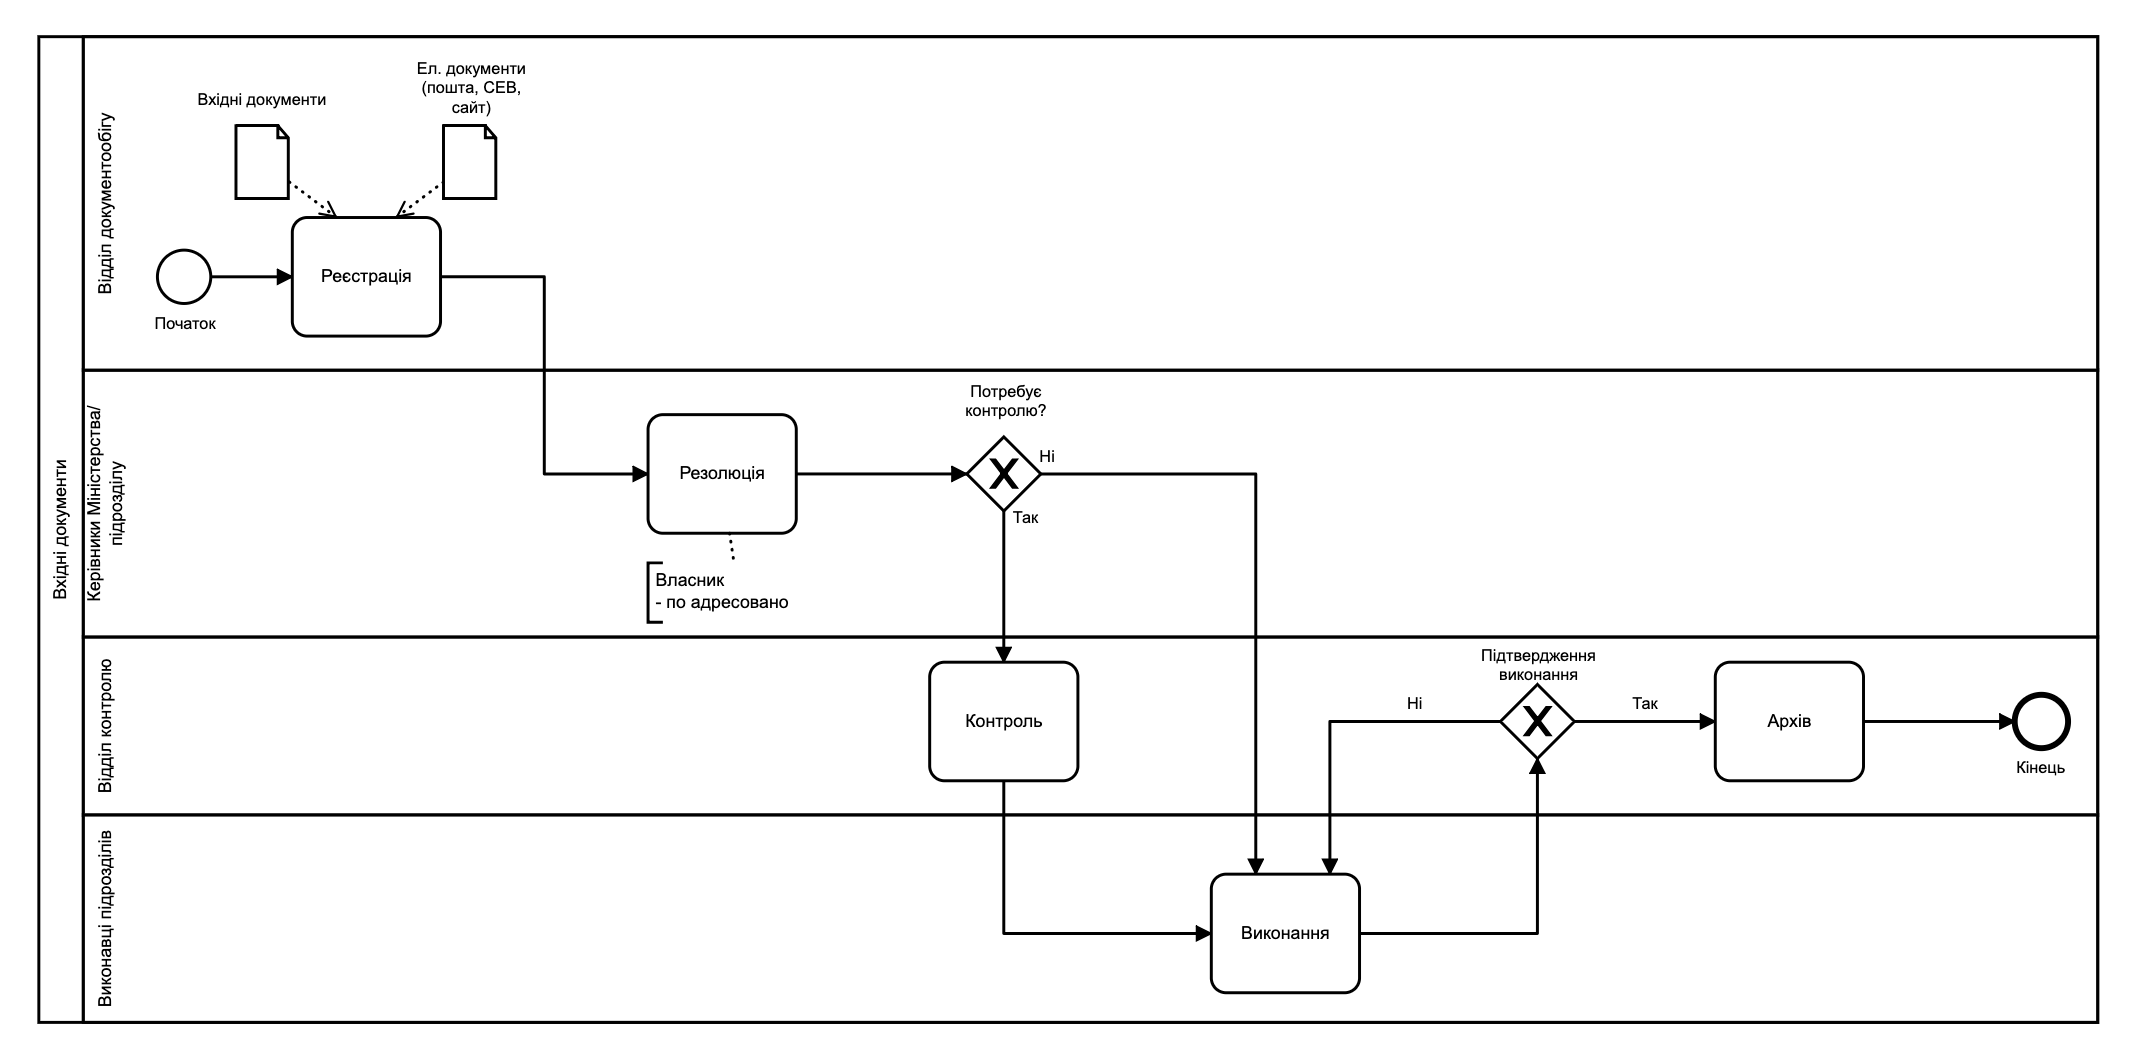
\includegraphics[scale=0.27]{inputDoc.png}}
\caption{Бізнес-процес вхідних докумнетів}
\end{figure}

\subsubsection{Вихідні документи}

\begin{figure}[!htbp]
\centerline{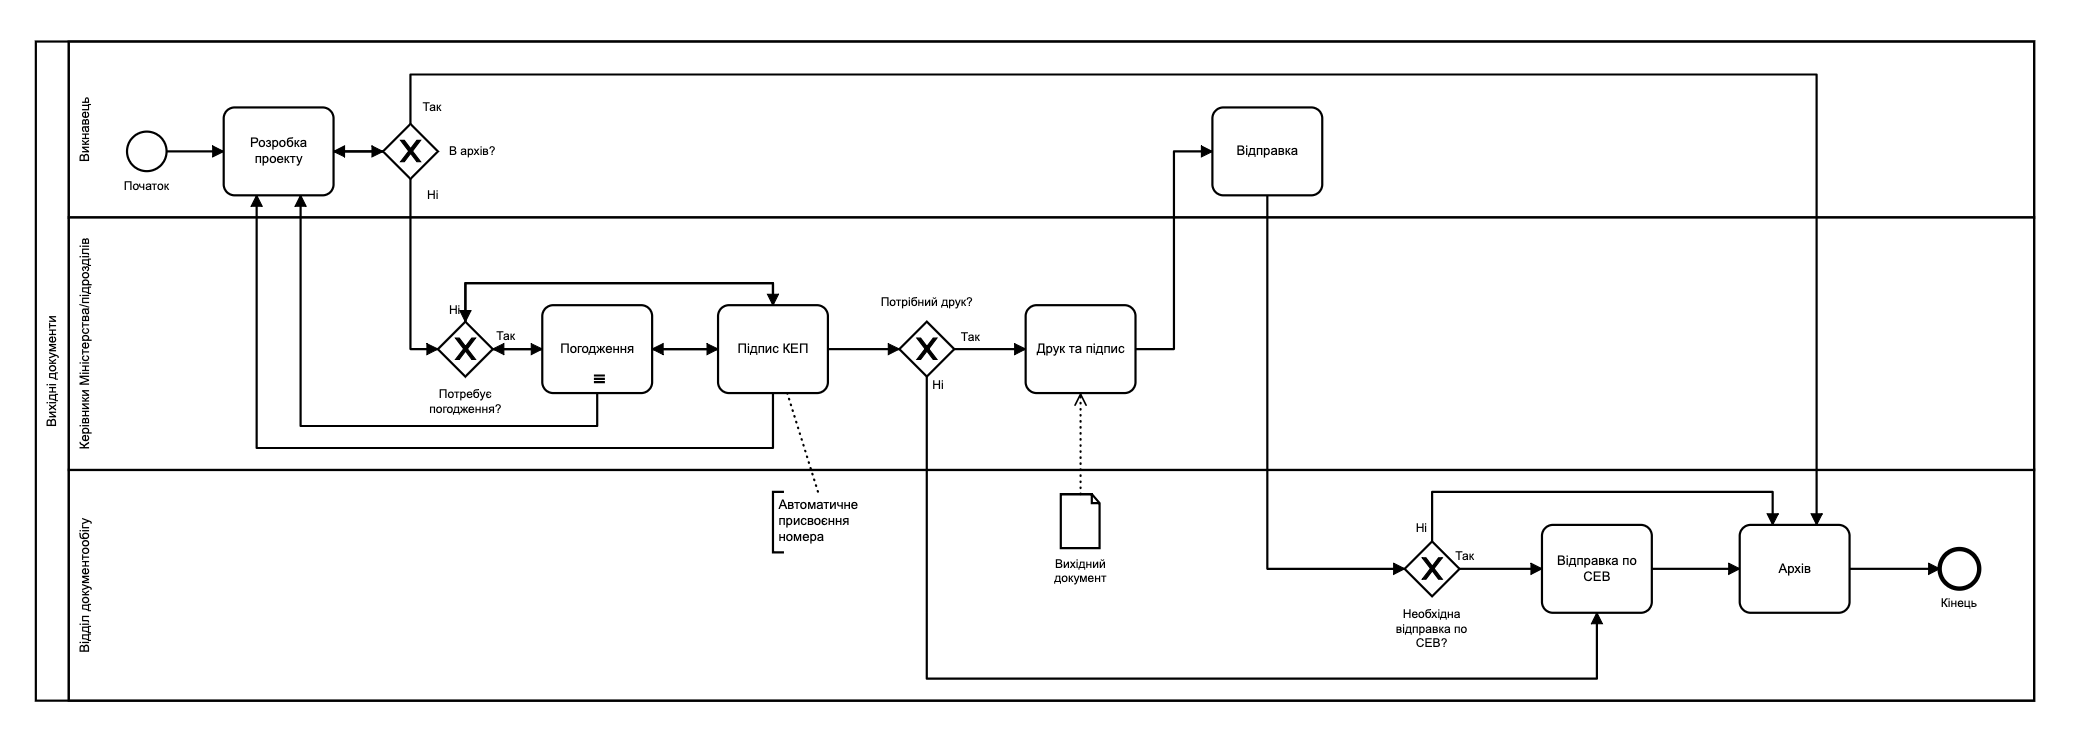
\includegraphics[scale=0.27]{outputDoc.png}}
\caption{Бізнес-процес вихідних докумнетів}
\end{figure}

Вихідні документи створюються в підрозділах (ініціатор документа).
Вихідні документи можуть виникати з ініціативи співробітників
Міністерства або ж в результаті обробки вхідних документів.
Якщо вихідний документ пов'язаний з вхідним документом, то
відповідальному працівнику необхідно вказати посилання на
пов'язаний документ. Обробка документів виконується по
одному бізнес-процесу, незалежно від місця виникнення документа.
В системі реєструється проект вихідного документа,
який повинен бути погоджений з переліком погоджуючих осіб.
Після підпису фінальним підписантом, документу присвоюється
номер та виконується відправка.

\subsubsection{Внутрішні документи}

Внутрішні документи можуть вводитися всіма учасниками документообігу.
Виділяються наступні основні бізнес-процеси внутрішніх
документів: «Доповідна записка», «Лист».

\begin{figure}[!htbp]
\centerline{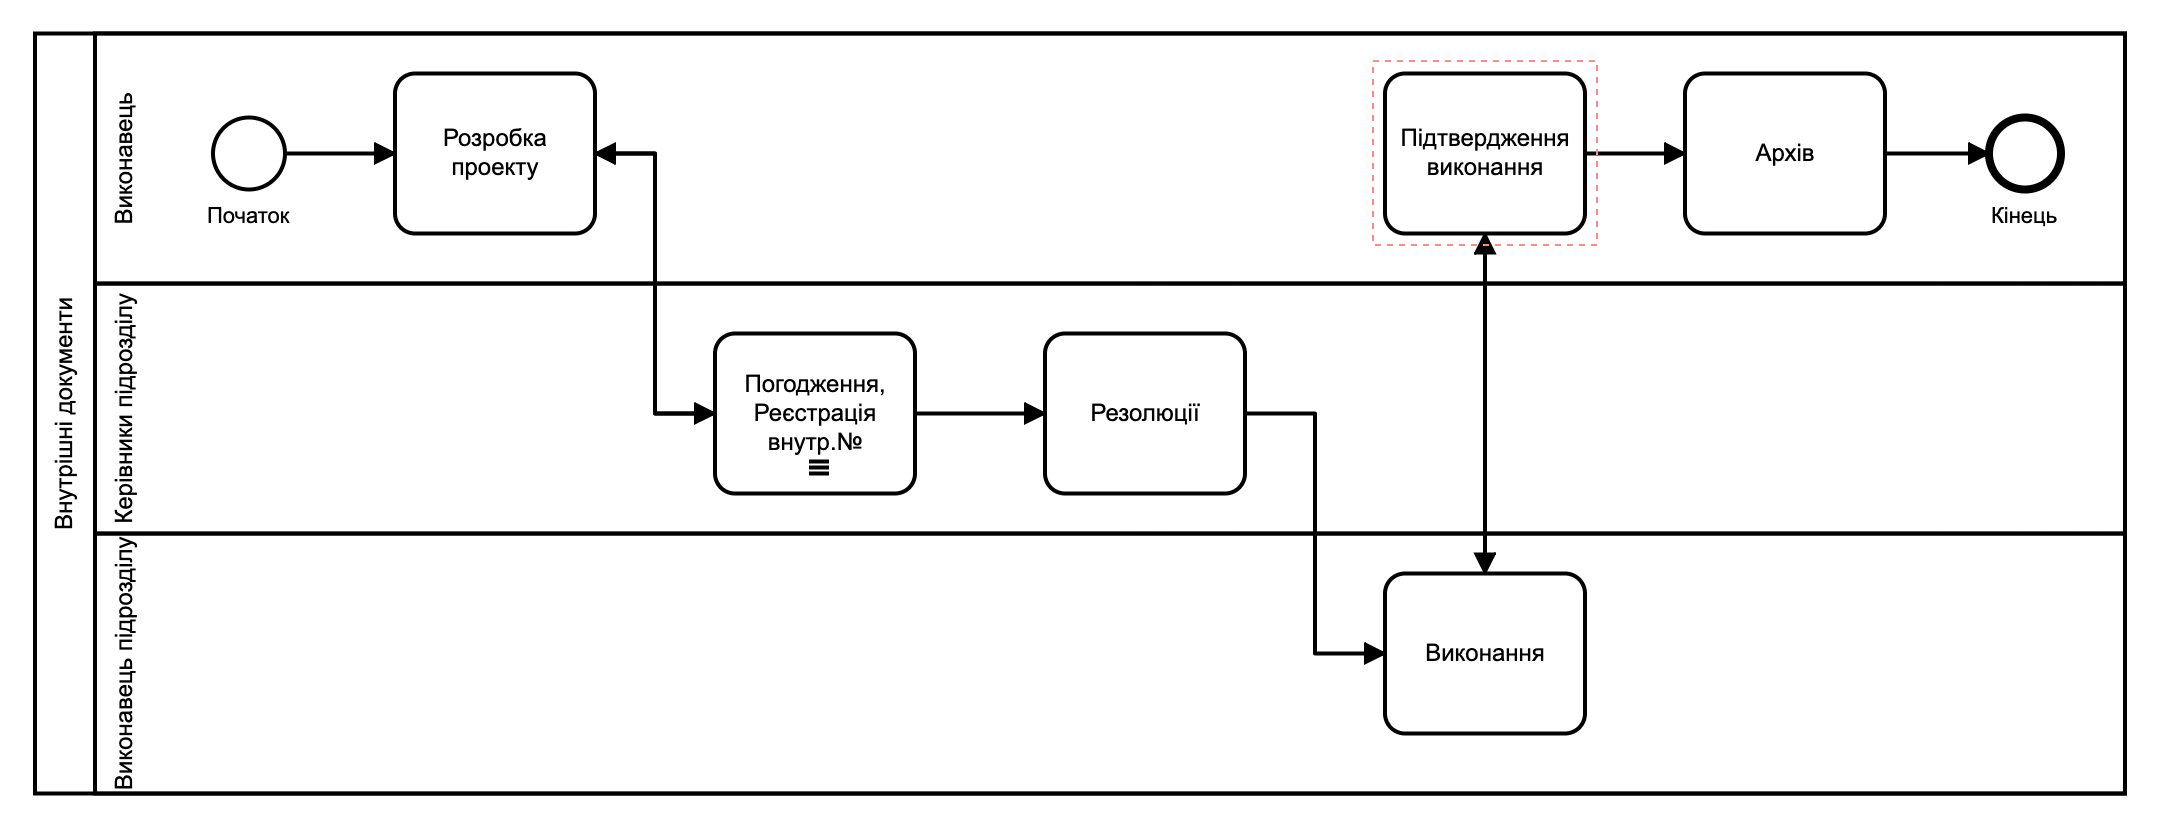
\includegraphics[scale=0.27]{internalDoc.png}}
\caption{Бізнес-процес внутрішніх докумнетів}
\end{figure}

\subsubsection{Організаційно-розпорядні документи}

\begin{figure}[!htbp]
\centerline{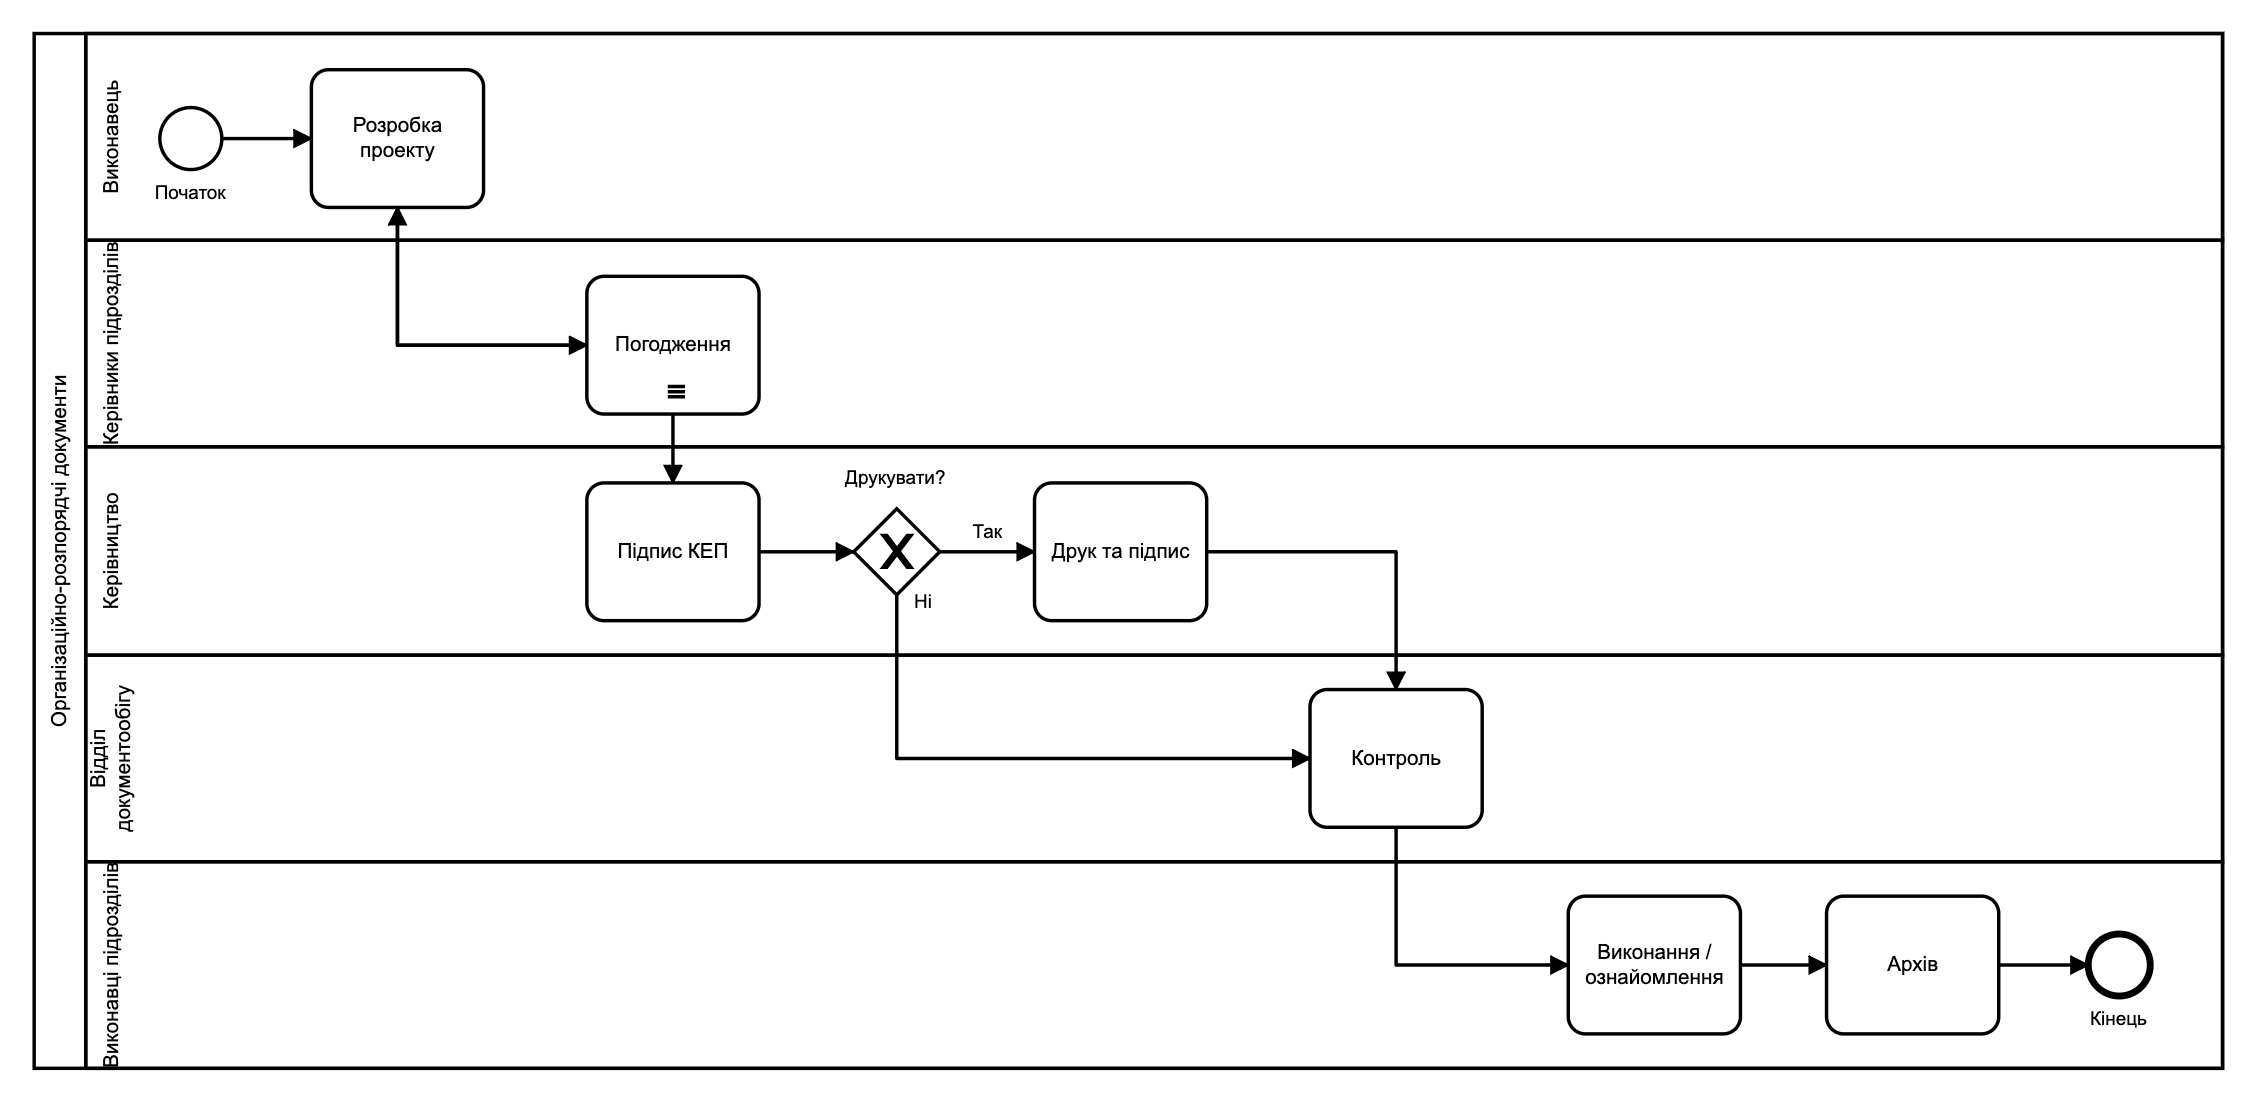
\includegraphics[scale=0.25]{orgDoc.png}}
\caption{Бізнес-процес організаційно-розпорядних докумнетів}
\end{figure}

\subsubsection*{Розробка проекту документа}

На даному етапі розробляється електронний проект документа:
заповнюються всі необхідні реквізити в електронній картці документа,
після збереження електронної картки автоматично прикріплюється шаблон
документа як оригінал. Виконавець вносить вміст документа в оригінал
і зберігає його. Ініціатор додає всіх виконавців, кому адресований
наказ. По полю «Адресовано» автоматично будуть створені задачі на виконавців.
Далі необхідно передати документ на наступний крок.

\subsubsection*{Погодження}

На даному кроці виконується погодження документа особами, які були вказані
Виконавцем при створенні проекту документа.
Обов'язковою умовою передачі документа на наступний етап - позитивне погодження
від ВСІХ погожуючих осіб. Інакше далі передати документ неможливо. Якщо один
з візуючих відхилив документ (при цьому вноситься коментар з причинами
відхилення і зауваженнями до документа) - в даному випадку документ
повертається на першу стадію Виконавцю на доопрацювання.
Якщо всі особи погодили документ - він автоматично передається на наступну стадію.
Після погодження документу можна сформувати Аркуш погодження у вигляді друкованої форми.

\subsubsection*{КЕП}

На даній стадії документ підписується в електронному вигляді Керівництвом Міністерства.
Під час цього документу присвоюється реєстраційний номер.
У разі налагодження СЕД на використання QR-коду, він розміром
21 на 21 мм розміщується в нижньому лівому куті першої сторінки документа.
У разі налагодження СЕД на використання штрих-коду, він розміщується у правому кутку нижнього поля першої сторінки документа.

\subsubsection*{Підпис}

Після підписання організаційно-розпорядчого документу, у разі
необхідності створення паперового варіанту уповноважена особа
служби (помічник) Міністра/заступника міністра/державного секретаря
роздруковує документ та надає на підпис керівнику.
Якщо організаційно-розпорядчийдокумент підписано керівником
підрозділу, то при необхідності документ роздруковує виконавець.

\subsubsection*{Постановка на контроль}

На даному етапі контролюючий СП перевіряє завдання по документу,
при необхідності здійснює постановку на контроль, та періодичність.
Документи і задачі на контролі незалежно від кроку опрацювання
документа доступні за окремим фільтром, їх можна відстежувати
незалежно від того, на якій стадії знаходиться документ,
контролювати виконання, проводити аналіз, і т.д.

\subsubsection*{Виконання/Ознайомлення}

На даному етапі контролюючий СП перевіряє завдання по документу,
при необхідності здійснює постановку на контроль, та періодичність.
Документи і задачі на контролі незалежно від кроку опрацювання
документа доступні за окремим фільтром, їх можна відстежувати
незалежно від того, на якій стадії знаходиться документ, контролювати
виконання, проводити аналіз, і т.д.

\subsubsection*{Цифровий шифровий архів}

Після ознайомлення документ переходить в Архів, який додатково накладає
підписи КЕП Архіву та утримує істрорію всіх проміжних сертифікатів АЦСК до ЦЗО..

\subsubsection{Звернення громадян}

\begin{figure}[!htbp]
\centerline{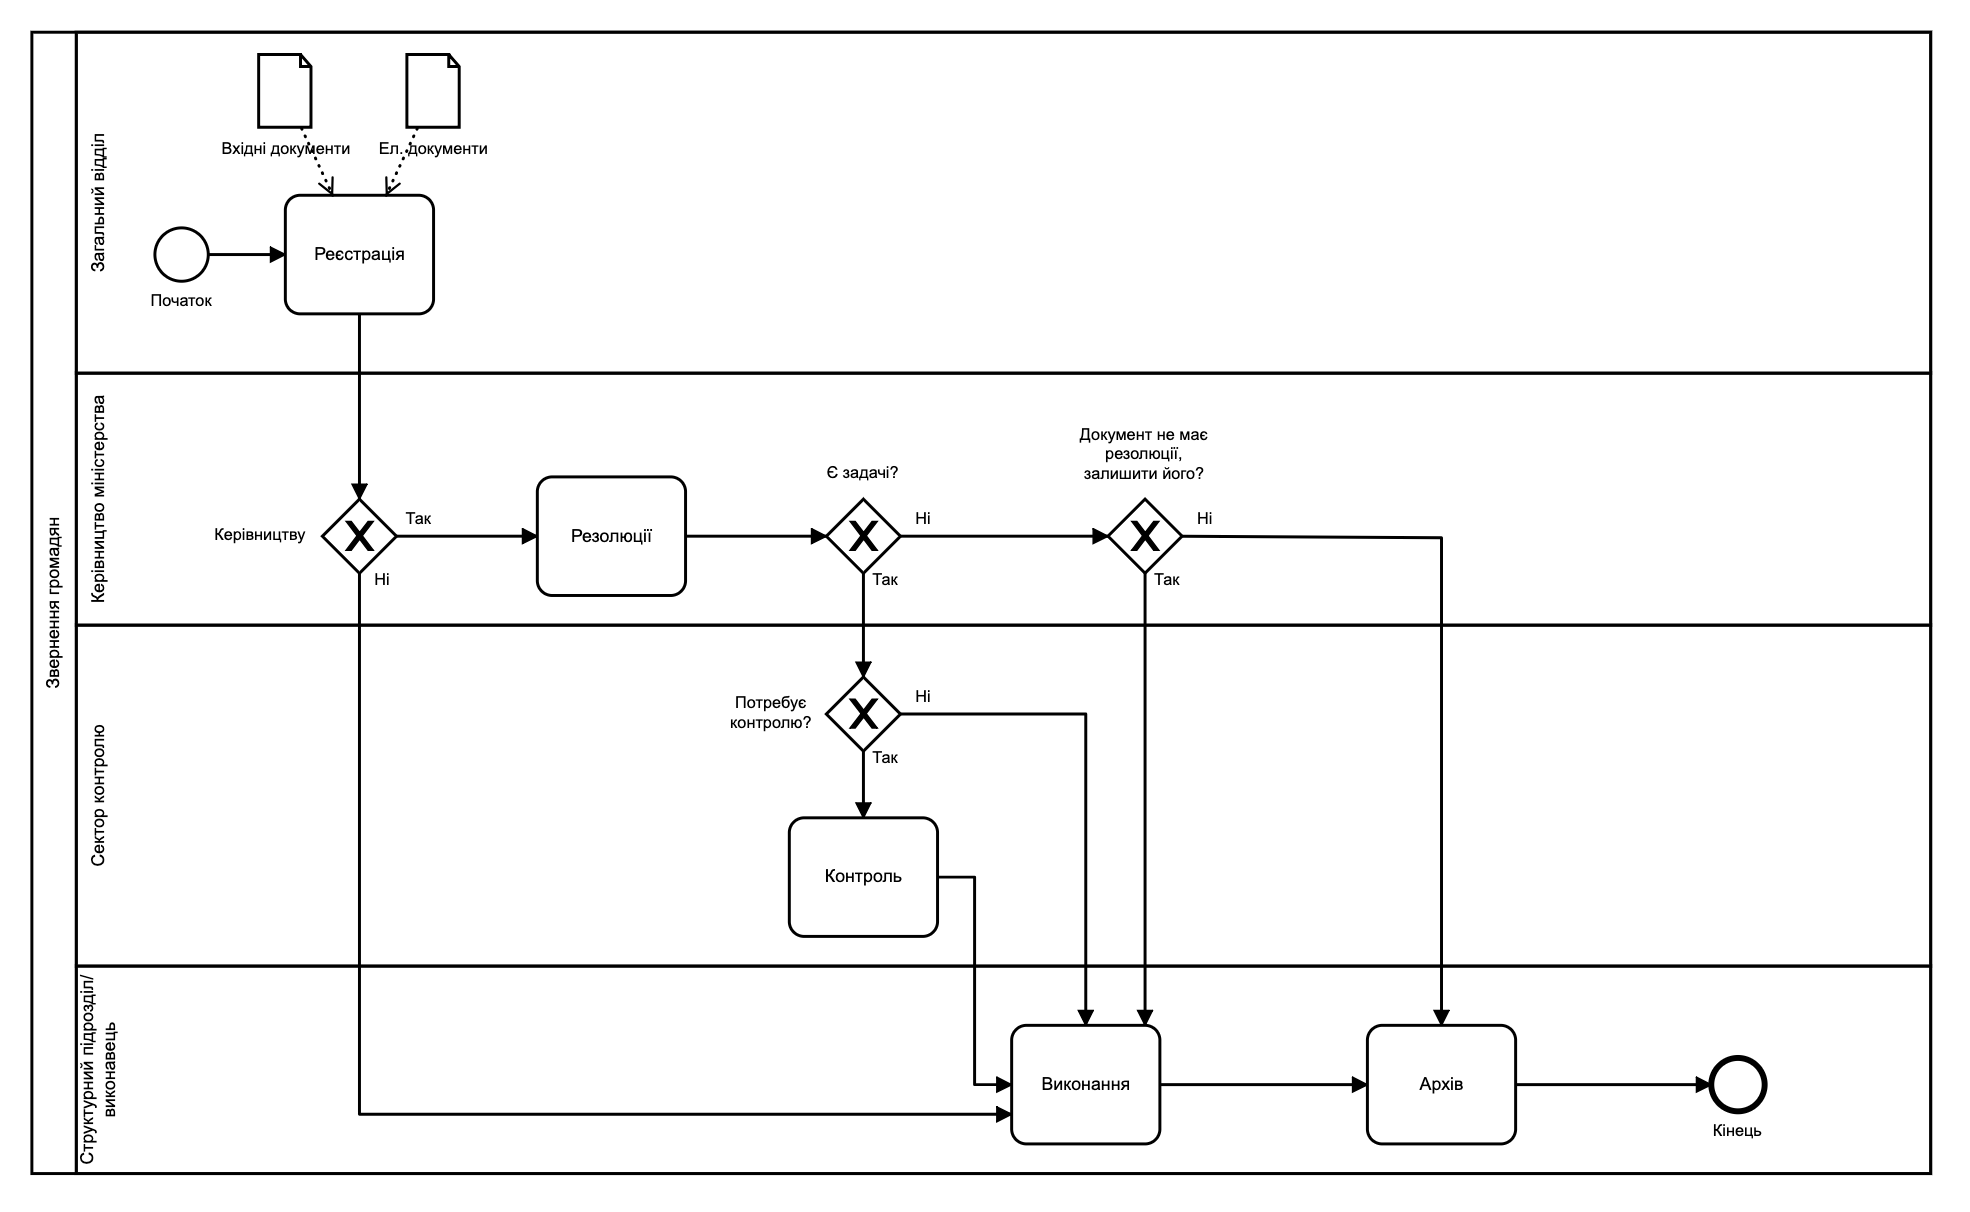
\includegraphics[scale=0.3]{citizenInquire.png}}
\caption{Бізнес-процес звернення громадян}
\end{figure}

\newpage
\subsection{Елементи}

Тут зібрана мінімальна кількість бізнес-форм, специфічних для CRM СЕД,
яка необхідня для забезпечення реалізації функціональних вимог замовника.

\subsubsection{Календар}

Календар взятий з бібліотеки NITRO, проте потребує додаткової стилізації.

\begin{figure}[!htbp]
\centerline{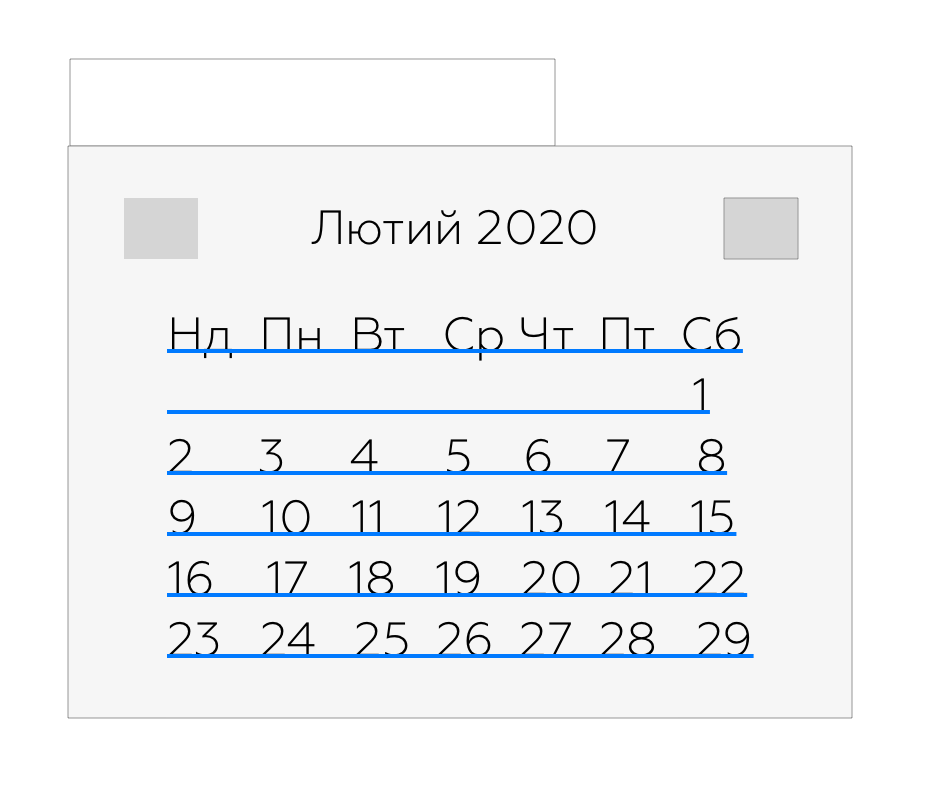
\includegraphics[scale=0.4]{calendar.png}}
\caption{Контрольний елемент Календар}
\end{figure}

\newpage
\subsubsection{Пошук по довільним фідам}

Для забезпечення пошуку по словникам та бізнес-об'єктами системе
передбачається створення спеціалізованого скалярного комбо-пошуку по довільним
фідам в сховищі даних. Наприклад: Співробітники, Населені пункти КОАТУУ, тощо.

\begin{figure}[!htbp]
\centerline{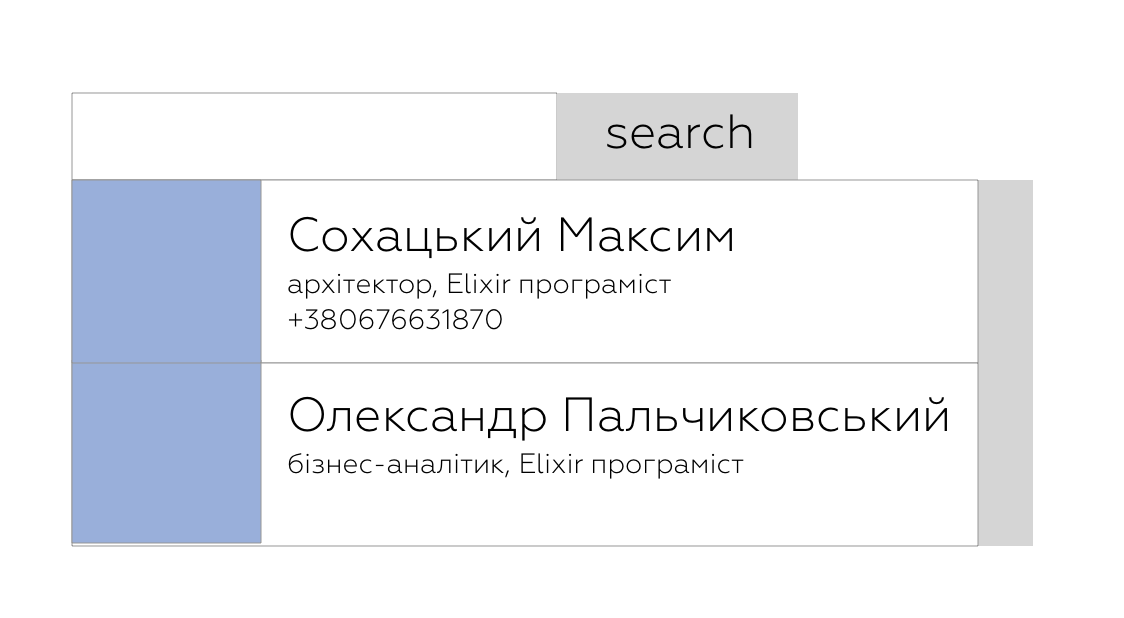
\includegraphics[scale=0.3]{comboLookup.png}}
\caption{Контрольний елмент віддаленого пошуку по базі даних}
\end{figure}

\subsubsection{Форма редагування та пошуку}

Для кожного типу документу в системі реєструються дві форми: форма пошуку
та форма редагування (вона ж форма створення нового). Наявність двох форм
вмотивована відмінністю валідаторі: для пошуку валідатори повинні дозволяти пусті поля,
позаяк для редагування валідатори повинні перевіряти валідність полів бізнес-об'єктів.

\begin{figure}[!htbp]
\centerline{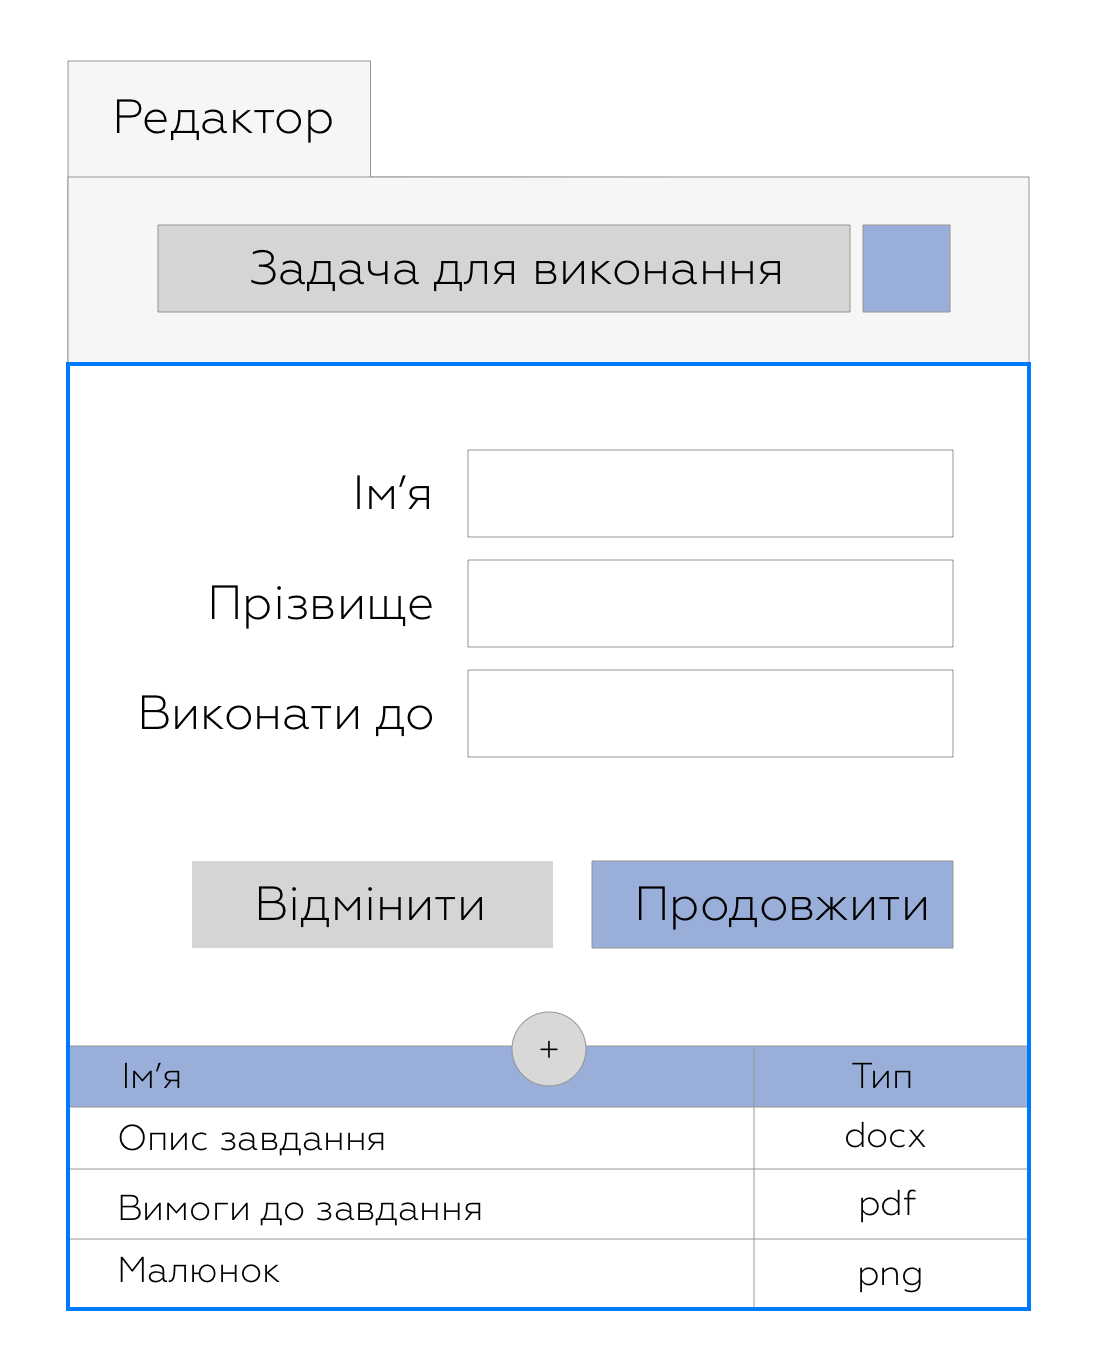
\includegraphics[scale=0.3]{editForm.png}}
\caption{Контрольний елемент редагування документу та підлеглих файлів}
\end{figure}

\newpage
\subsubsection{Управління бізнес процесом}

Для управління завдання, доступу до документів процесу, створення нових документів в процесі,
візування, підпису, проштовху документів по бізнес-процесу використовується стандартний
контрольний елемент управління бізнес-процесом.

\begin{figure}[!htbp]
\centerline{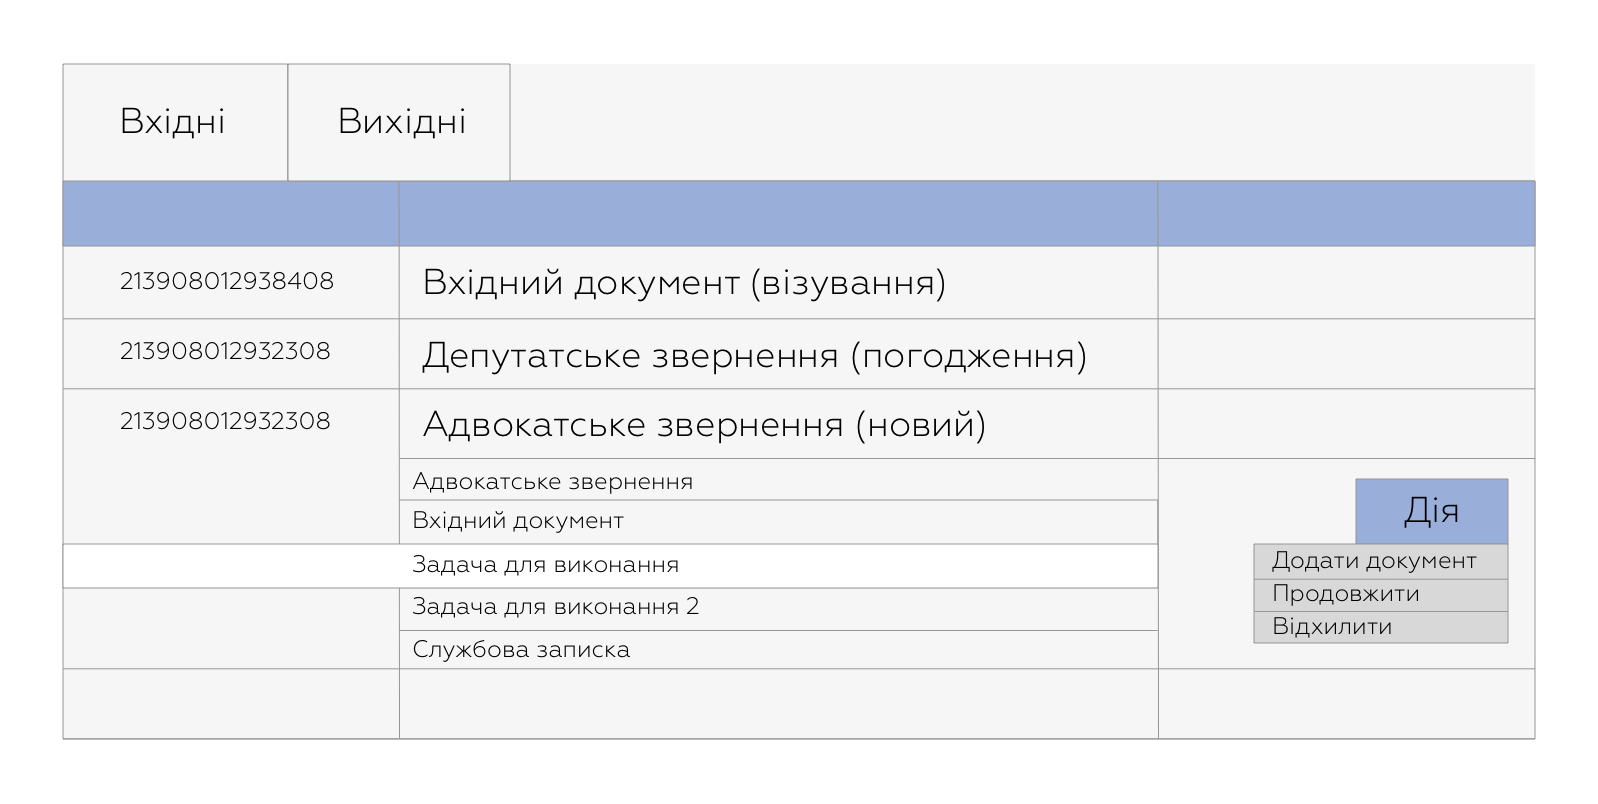
\includegraphics[scale=0.3]{bpeControl.png}}
\caption{Контрольний елемент управління бізнес-процесами}
\end{figure}

\subsubsection{Документи в бізнес-процесах}

При навігації по дукументам процесу передбачається миттєве відображення підлеглого
документа в лівій панелі головної сторінки користувацького інтерфейсу.

\begin{figure}[!htbp]
\centerline{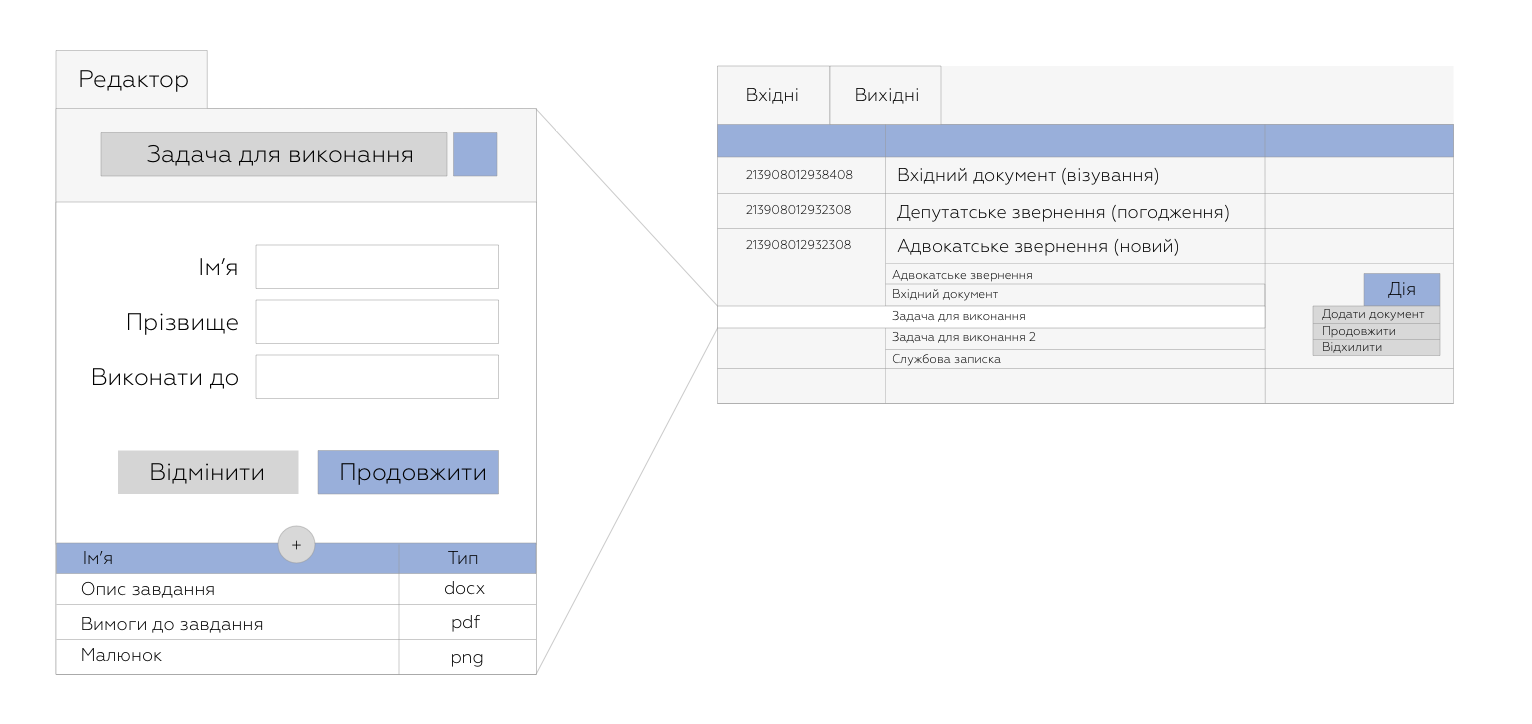
\includegraphics[scale=0.4]{searchBpe.png}}
\caption{Навігація по документам бізнес-процесу}
\end{figure}

\newpage
\subsubsection{Використання контролів на формах}

Приклад використання контрольного елементу довільного пошуку на формах.

\begin{figure}[!htbp]
\centerline{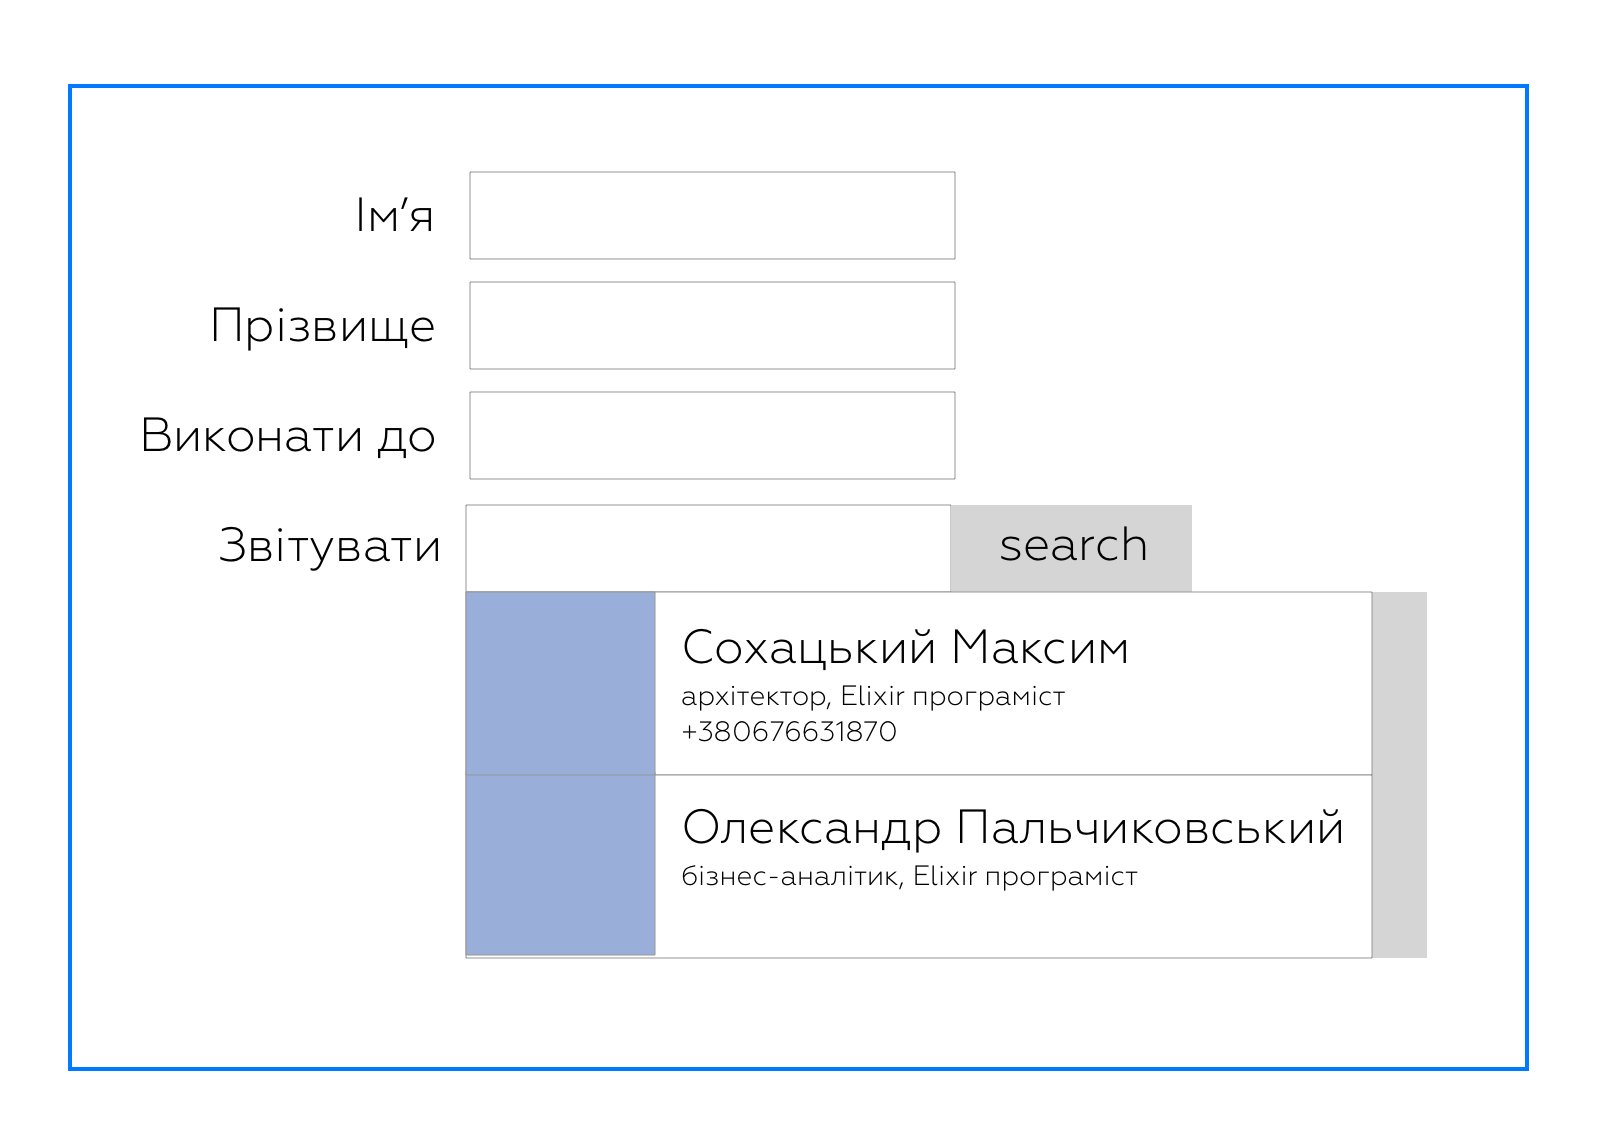
\includegraphics[scale=0.3]{comboLookupForm.png}}
\caption{Приклад використання контрольних елементів на формах}
\end{figure}

\subsubsection{Контрольний елемент КОАТУУ}

Приклад використання контрольного елементу КОАТУУ.

\begin{figure}[!htbp]
\centerline{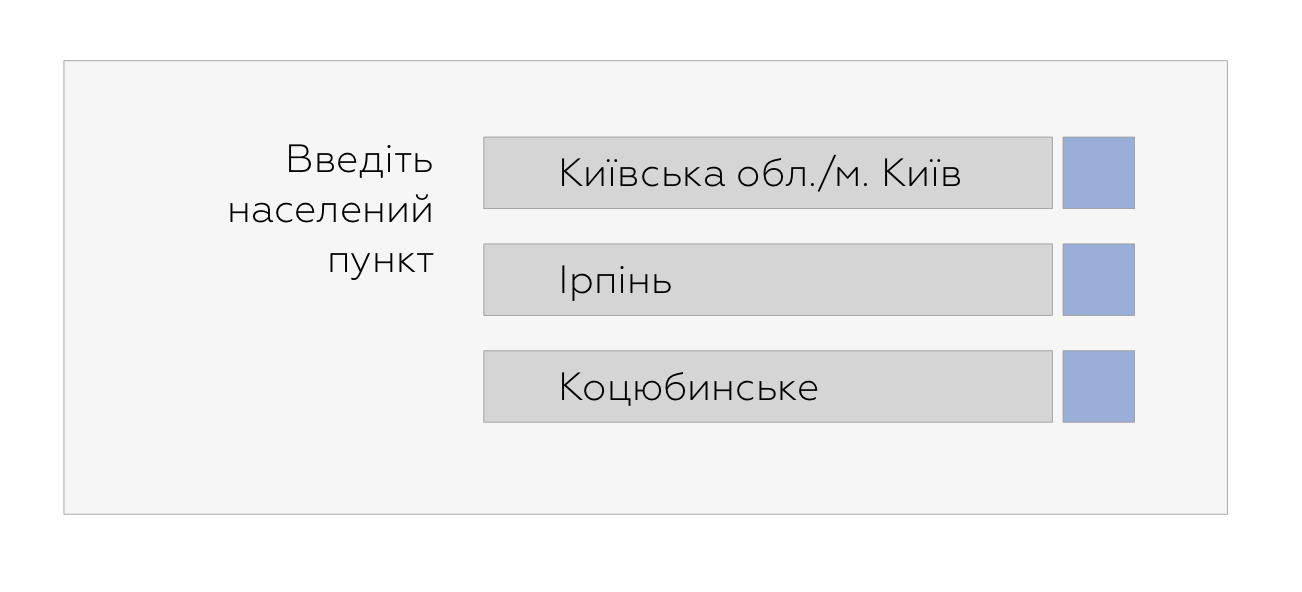
\includegraphics[scale=0.3]{koatuu.png}}
\caption{Приклад використання контрольного елементу КОАТУУ}
\end{figure}

\newpage
\subsection{Редактори}

Тут будуть перелічені контроллери сторінок, кожна з яких є SPA веб додатком.

\subsubsection{Вхід в систему}

Сторінка входу в систему з використанням ЕЦП.

\begin{figure}[!htbp]
\centerline{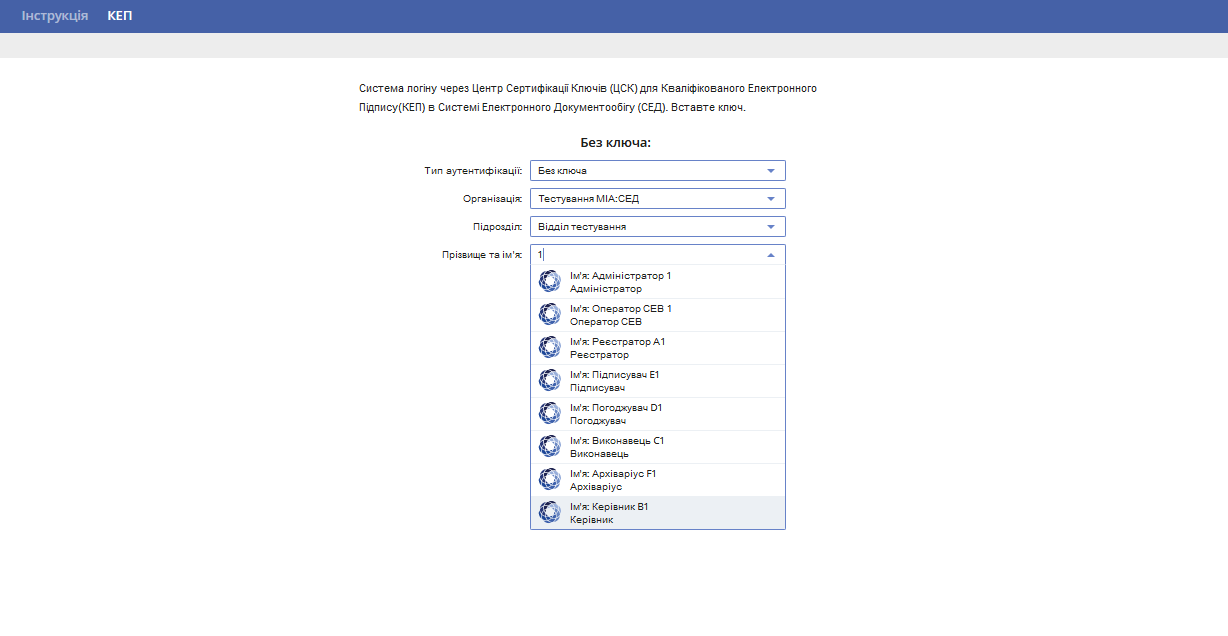
\includegraphics[scale=0.4]{ldap.png}}
\caption{Сторінка входу в систему}
\end{figure}

\newpage
\subsubsection{Робота з документами}

Головна сторінка системи для роботи з документами в бізнес-процесах.

\begin{figure}[!htbp]
\centerline{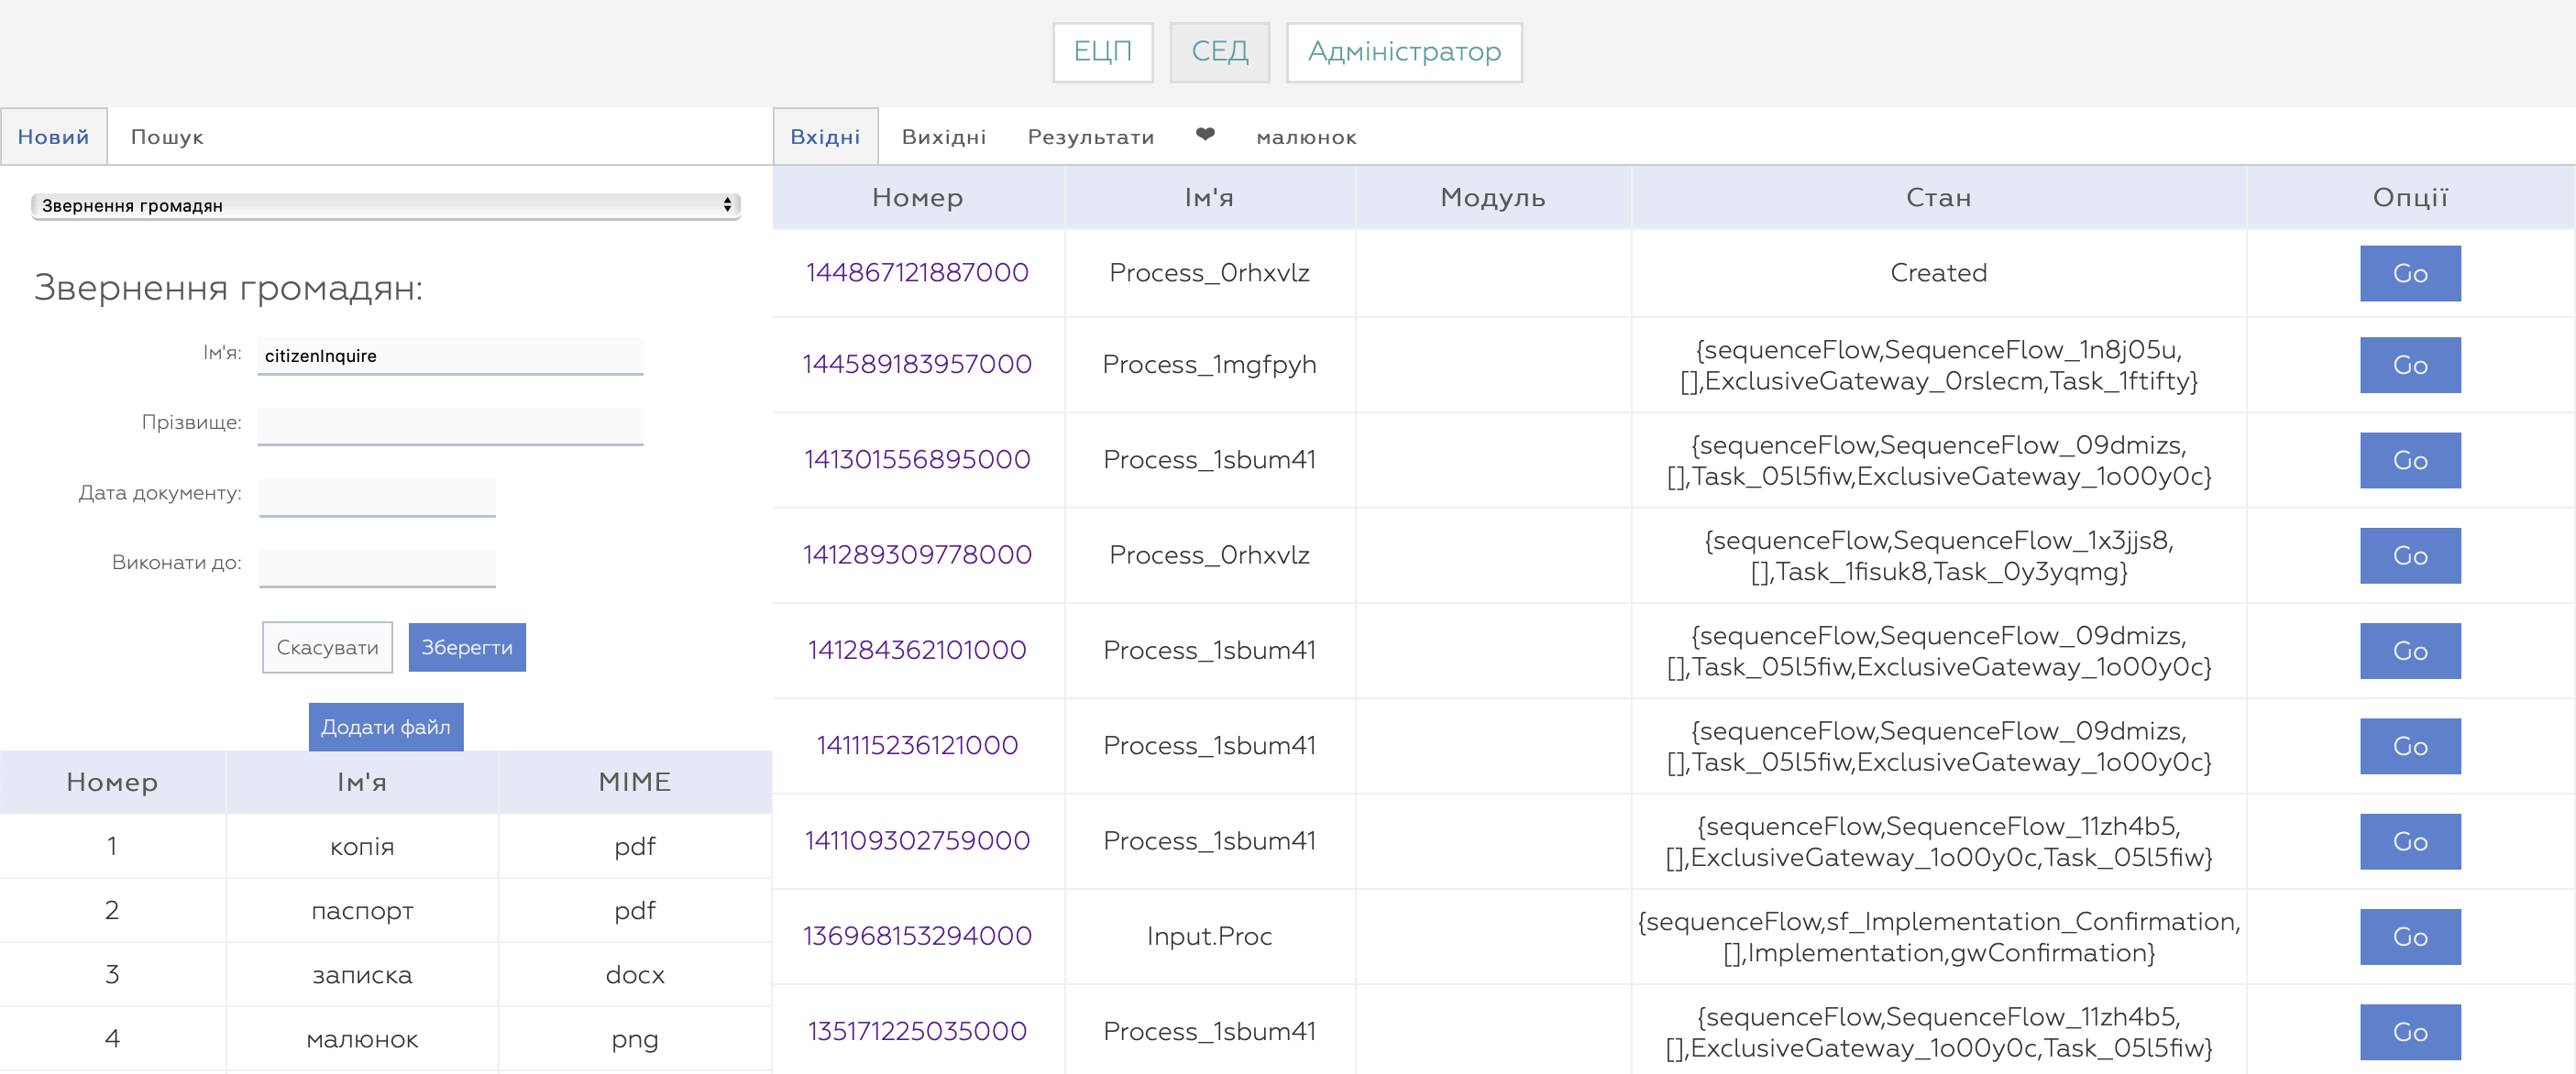
\includegraphics[scale=0.2]{crm.png}}
\caption{Сторінка роботи з документами}
\end{figure}

При навігації по дукументам процесу передбачається миттєве відображення підлеглого
документа в лівій панелі головної сторінки користувацького інтерфейсу.

\begin{figure}[!htbp]
\centerline{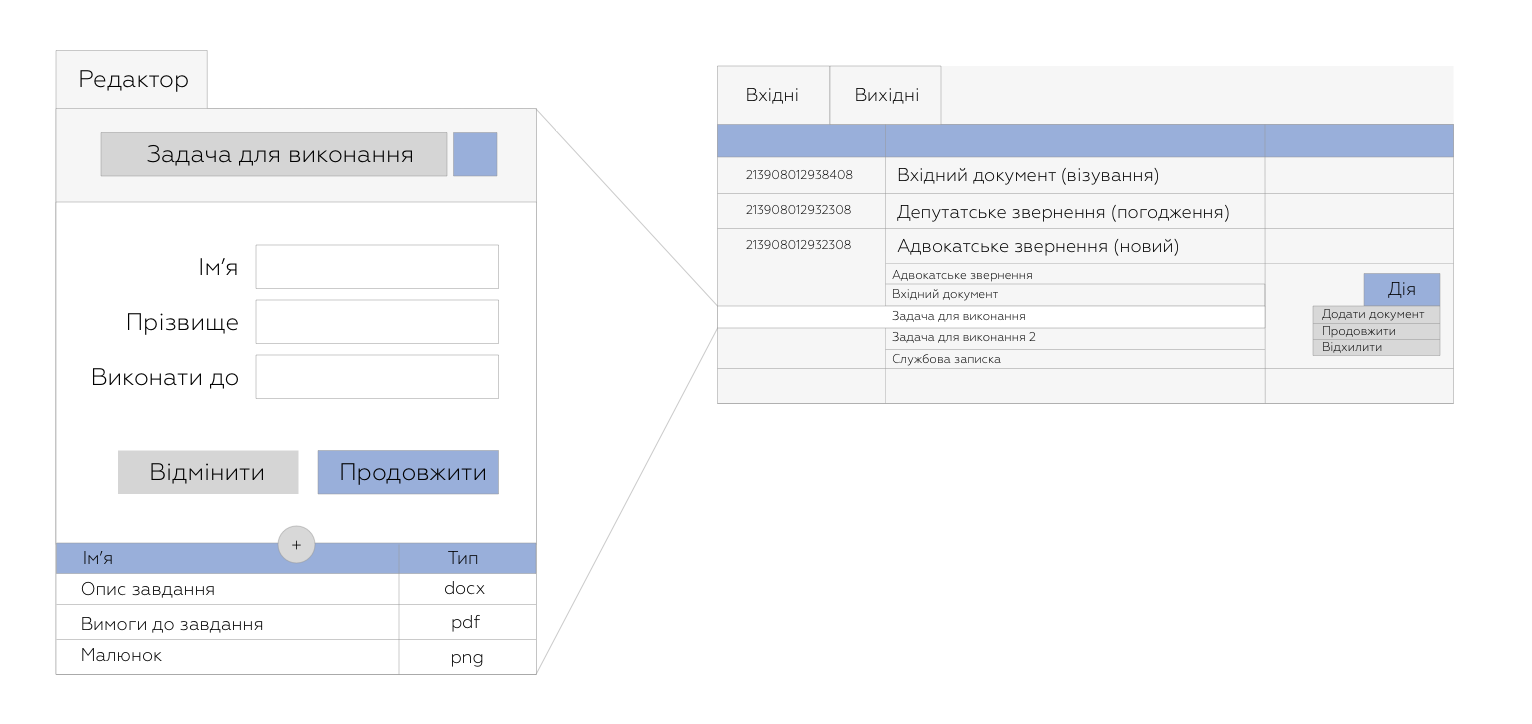
\includegraphics[scale=0.4]{searchBpe.png}}
\caption{Навігація по підлеглим документам}
\end{figure}

\newpage
\subsection{Конструктор}

Тут представлені адміністративні сторінки управління системою.

\subsubsection{Бізнес-об'єкти}

Глобальний каталог усіх бізнес-об'єктів системи.

\subsubsection{Бізнес-процеси}

Перелік усіх зареєстрованих бізнес-процесів в системі, та можливість їх тестування.

\subsubsection{Бізнес-форми}

Перелік усіх форм документів та бізнес-форм користувача, зареєстрованих в системі.



